\documentclass[aspectratio=169,10pt]{beamer}

% Shared Beamer setup for Fall 2026 course slides.
% Clean Cal Poly-inspired theme: no custom class files or uncommon packages.
\mode<presentation>{
  \usetheme{default}
  \usefonttheme{professionalfonts}
}

\definecolor{CalPolyGreen}{HTML}{154734}
\definecolor{CalPolyGold}{HTML}{BD8B13}
\definecolor{CalPolySage}{HTML}{7FA28F}
\definecolor{CalPolyMint}{HTML}{DDF1E7}
\definecolor{CalPolySand}{HTML}{A29F86}
\definecolor{CalPolyBeige}{HTML}{EFEEDE}
\definecolor{DeckInk}{HTML}{1F2933}
\definecolor{DeckMuted}{HTML}{5F6B7A}
\definecolor{DeckSoft}{HTML}{F7F7F5}

\setbeamersize{text margin left=0.55in,text margin right=0.55in}
\setbeamercolor{normal text}{fg=DeckInk,bg=white}
\setbeamercolor{structure}{fg=CalPolyGreen}
\setbeamercolor{title}{fg=white}
\setbeamercolor{frametitle}{fg=CalPolyGreen,bg=white}
\setbeamercolor{block title}{bg=CalPolySage,fg=white}
\setbeamercolor{block body}{bg=CalPolyMint,fg=black}
\setbeamercolor{alerted text}{fg=CalPolyGold}

\setbeamerfont{title}{size=\Huge,series=\bfseries}
\setbeamerfont{frametitle}{size=\Large,series=\bfseries}
\setbeamerfont{block title}{size=\normalsize,series=\bfseries}

\setbeamertemplate{navigation symbols}{}
\setbeamertemplate{itemize item}{\color{CalPolyGold}$\blacktriangleright$}
\setbeamertemplate{itemize subitem}{\color{CalPolyGreen}$\bullet$}
\setbeamertemplate{footline}{
  \hfill{\color{DeckMuted}\scriptsize\insertframenumber/\inserttotalframenumber}
  \hspace{0.18in}\vspace{0.12in}
}
\setbeamertemplate{frametitle}{
  \vspace{0.18in}
  \hspace{0.02in}\insertframetitle\par
  \vspace{0.08in}
  \noindent\makebox[\linewidth][l]{%
    {\color{CalPolyGold}\rule{0.55in}{2pt}}%
    {\color{CalPolyGreen}\rule{\dimexpr\linewidth-0.55in\relax}{2pt}}%
  }
}

\newcommand{\CourseNumber}{Course}
\newcommand{\CourseTitle}{Course Title}
\newcommand{\LectureNumber}{0}
\newcommand{\LectureTitle}{Lecture Title}
\newcommand{\LectureDate}{Date}
\newcommand{\CourseUnit}{Unit}

\newcommand{\coursenumber}[1]{\renewcommand{\CourseNumber}{#1}}
\newcommand{\coursetitle}[1]{\renewcommand{\CourseTitle}{#1}}
\newcommand{\lecturenumber}[1]{\renewcommand{\LectureNumber}{#1}}
\newcommand{\lecturetitle}[1]{\renewcommand{\LectureTitle}{#1}}
\newcommand{\lecturedate}[1]{\renewcommand{\LectureDate}{#1}}
\newcommand{\courseunit}[1]{\renewcommand{\CourseUnit}{#1}}

\author{Kirk Duran}
\institute{California Polytechnic State University, San Luis Obispo}
\date{\LectureDate}

\newcommand{\makedecktitle}{
  \begingroup
  \setbeamercolor{background canvas}{bg=CalPolyGreen}
  \begin{frame}[plain]
    \vfill
    \begin{center}
      {\usebeamerfont{title}\color{white}\LectureTitle\par}
      \vspace{0.18in}
      {\Large\color{white}Lecture \LectureNumber\par}
    \end{center}
    \vfill
    \noindent{\color{white}\rule{\linewidth}{1.2pt}}\par
    \vspace{0.08in}
    \noindent\colorbox{CalPolyGold}{\makebox[0.24\linewidth][c]{\color{white}\Large\CourseNumber}}
    \hspace{0.12in}{\color{white}\Large Kirk Duran}
  \end{frame}
  \endgroup
}

\newenvironment{keyidea}{\begin{block}{Key idea}}{\end{block}}
\newenvironment{activity}{\begin{block}{In class}}{\end{block}}
\newenvironment{cpdefinition}{\begin{block}{Definition}}{\end{block}}
\newenvironment{exampleblockcp}{
  \begingroup
  \setbeamercolor{block title}{bg=CalPolySand,fg=white}
  \setbeamercolor{block body}{bg=CalPolyBeige,fg=black}
  \begin{block}{Example}
}{
  \end{block}
  \endgroup
}

\newcommand{\imageplaceholder}[2][0.3in]{%
  \noindent\makebox[\linewidth][c]{%
    \fcolorbox{CalPolySage}{CalPolyBeige}{%
      \parbox[c][#1][c]{0.86\linewidth}{%
        \centering
        {\color{DeckMuted}\scriptsize Image placeholder: }%
        {\color{DeckInk}\scriptsize\ttfamily\detokenize{#2}}%
      }%
    }%
  }%
}

\newcommand{\sectionframe}[1]{
  \begingroup
  \setbeamercolor{background canvas}{bg=CalPolyGreen}
  \begin{frame}[plain]
    \vfill
    {\color{white}\LARGE\bfseries #1\par}
    \vspace{0.18in}
    {\color{CalPolyGold}\rule{0.22\paperwidth}{3pt}}
    {\color{white}\rule{0.62\paperwidth}{3pt}}
    \vfill
  \end{frame}
  \endgroup
}

\newcommand{\placeholdernote}{
  \begin{block}{Placeholder}
    Replace these bullets with the final lecture material, examples, and in-class activities.
  \end{block}
}


\usepackage{tikz}
\usetikzlibrary{arrows.meta,positioning,calc}

\graphicspath{{../assets/lecture-21/}}

\newcommand{\lectureimage}[2][1.75in]{%
  \IfFileExists{../assets/lecture-21/#2}{%
    \includegraphics[width=\linewidth,height=#1,keepaspectratio]{#2}%
  }{}%
}

\newcommand{\lectureplaceholder}[2][2.35in]{%
  \begin{center}
    \fbox{%
      \begin{minipage}[c][#1][c]{0.90\linewidth}
        \centering
        \small\textit{#2}
      \end{minipage}%
    }
  \end{center}%
}

\setbeamersize{text margin left=0.42in,text margin right=0.42in}

\coursenumber{CS 4880}
\coursetitle{Artificial Intelligence}
\lecturenumber{21}
\lecturetitle{Reasoning Over Time: State Estimation}
\lecturedate{October 14, 2026}
\courseunit{Temporal and Decision Reasoning}

\begin{document}

% Estimated pacing: 52--55 minutes
% Dynamic Bayesian networks: 8 min
% Filtering worked example + blow-up: 12 min
% Markov assumption + HMMs: 12 min
% Kalman filtering: 9 min
% Particle filtering + AMCL: 11 min
% Synthesis: 3 min

% -----------------------------------------------------------------------------
% Slide 1
% -----------------------------------------------------------------------------
\makedecktitle

\section{From Static Beliefs to Changing Worlds}

% -----------------------------------------------------------------------------
% Slide 2
% -----------------------------------------------------------------------------
\begin{frame}[shrink=10]{Last Time: The World Was Frozen}
  Bayesian networks let the robot reason about uncertainty in a single snapshot:
  \[
    P(X_1,\ldots,X_n)=\prod_i P(X_i\mid Parents(X_i)).
  \]

  But a delivery robot does not live in a snapshot.

  \begin{itemize}
    \item the robot moves;
    \item pedestrians move;
    \item wheel odometry drifts;
    \item sensor readings arrive continuously;
    \item yesterday's best estimate may be wrong now.
  \end{itemize}

  \begin{keyidea}
    Temporal reasoning asks how an agent should update uncertain beliefs as the hidden world changes over time.
  \end{keyidea}
\end{frame}

% -----------------------------------------------------------------------------
% Slide 3
% -----------------------------------------------------------------------------
\begin{frame}[shrink=10]{The Campus Robot Now Has a New Problem}
  The route planner says where the robot \emph{should} be.

  The robot still needs to estimate where it \emph{actually} is.

  \begin{columns}[T,onlytextwidth]
    \begin{column}{0.54\textwidth}
      At time $t$, the robot has:
      \begin{itemize}
        \item a previous belief about its state;
        \item a control command or odometry estimate;
        \item a new noisy sensor observation;
        \item uncertainty in both motion and sensing.
      \end{itemize}
    \end{column}
    \begin{column}{0.40\textwidth}
      \lectureimage[2.7in]{slide3.png}
    \end{column}
  \end{columns}

  \begin{keyidea}
    Planning chooses a route; state estimation determines where the robot believes it is while executing that route.
  \end{keyidea}
\end{frame}

% -----------------------------------------------------------------------------
% Slide 4
% -----------------------------------------------------------------------------
\begin{frame}[shrink=10]{A Dynamic Bayesian Network Adds Time}
  Duplicate the relevant random variables across time slices.

  \begin{center}
    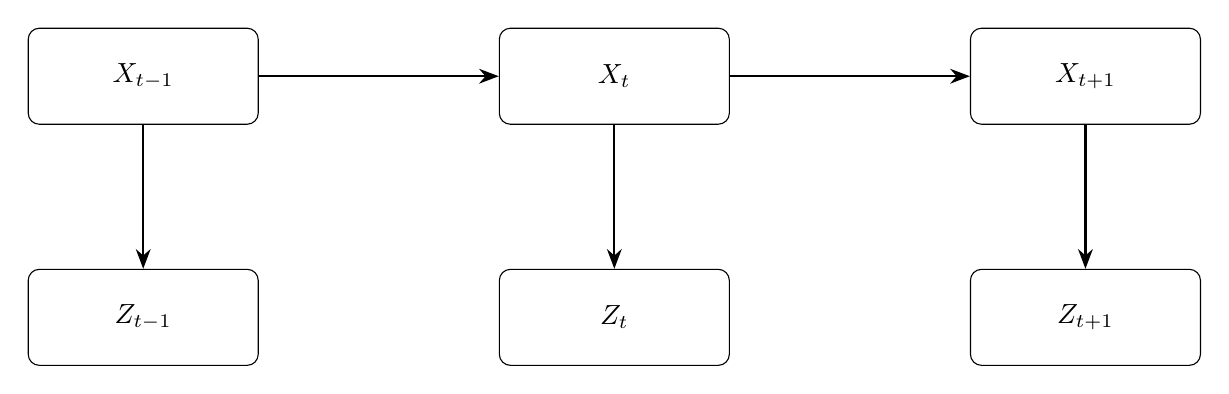
\begin{tikzpicture}[node distance=1.20in,every node/.style={draw,rounded corners,minimum width=1.15in,minimum height=0.48in,align=center}]
      \node (x0) {$X_{t-1}$};
      \node[right=of x0] (x1) {$X_t$};
      \node[right=of x1] (x2) {$X_{t+1}$};
      \node[below=0.72in of x0] (z0) {$Z_{t-1}$};
      \node[below=0.72in of x1] (z1) {$Z_t$};
      \node[below=0.72in of x2] (z2) {$Z_{t+1}$};
      \draw[-{Stealth[length=2.5mm]},thick] (x0)--(x1);
      \draw[-{Stealth[length=2.5mm]},thick] (x1)--(x2);
      \draw[-{Stealth[length=2.5mm]},thick] (x0)--(z0);
      \draw[-{Stealth[length=2.5mm]},thick] (x1)--(z1);
      \draw[-{Stealth[length=2.5mm]},thick] (x2)--(z2);
    \end{tikzpicture}
  \end{center}

  $X_t$ is the hidden state; $Z_t$ is the observation at time $t$.

  \begin{keyidea}
    A dynamic Bayesian network is a Bayesian network whose structure is repeated across time.
  \end{keyidea}
\end{frame}

% -----------------------------------------------------------------------------
% Slide 5
% -----------------------------------------------------------------------------
\begin{frame}[shrink=10]{For a Robot, Actions Also Affect the Next State}
  A useful robotics slice often contains a control input $U_t$:

  \begin{center}
    \begin{tikzpicture}[node distance=1.25in,every node/.style={draw,rounded corners,minimum width=1.10in,minimum height=0.48in,align=center}]
      \node (xm) {$X_{t-1}$};
      \node[right=of xm] (x) {$X_t$};
      \node[above=0.72in of x] (u) {$U_t$};
      \node[below=0.72in of x] (z) {$Z_t$};
      \draw[-{Stealth[length=2.5mm]},thick] (xm)--(x);
      \draw[-{Stealth[length=2.5mm]},thick] (u)--(x);
      \draw[-{Stealth[length=2.5mm]},thick] (x)--(z);
    \end{tikzpicture}
  \end{center}

  \[
    P(X_t\mid X_{t-1},U_t) \qquad \text{motion / transition model}
  \]
  \[
    P(Z_t\mid X_t) \qquad \text{sensor / observation model}
  \]

  \begin{keyidea}
    State estimation combines what motion predicts with what the sensors observe.
  \end{keyidea}
\end{frame}

% -----------------------------------------------------------------------------
% Slide 6
% -----------------------------------------------------------------------------
\begin{frame}[shrink=10]{The Temporal Joint Distribution}
  Under a first-order transition model and local observation model,
  \[
    P(x_{0:T},z_{1:T}\mid u_{1:T})
    =P(x_0)\prod_{t=1}^{T}
      P(x_t\mid x_{t-1},u_t)P(z_t\mid x_t).
  \]

  Every new time step adds:
  \begin{itemize}
    \item one new hidden state;
    \item one new observation;
    \item one transition factor;
    \item one observation factor.
  \end{itemize}

  \begin{keyidea}
    The model remains locally simple even as the complete trajectory becomes very large.
  \end{keyidea}
\end{frame}

% -----------------------------------------------------------------------------
% Slide 7
% -----------------------------------------------------------------------------
\begin{frame}[shrink=10]{Temporal Models Support Different Questions}
  \begin{center}
    \renewcommand{\arraystretch}{1.35}
    \begin{tabular}{l|l|l}
      \textbf{Task} & \textbf{Query} & \textbf{Question} \\\hline
      Filtering & $P(X_t\mid z_{1:t})$ & Where am I now? \\
      Prediction & $P(X_{t+k}\mid z_{1:t})$ & Where might I be later? \\
      Smoothing & $P(X_k\mid z_{1:t}),\;k<t$ & Where was I then? \\
      Most likely sequence & $\arg\max x_{1:t}P(x_{1:t}\mid z_{1:t})$ & What path most likely occurred? \\
    \end{tabular}
  \end{center}

  Today we focus on \textbf{filtering / state estimation}.

  \begin{keyidea}
    Filtering is online inference: estimate the current hidden state from all evidence observed so far.
  \end{keyidea}
\end{frame}

\section{Filtering: Exact State Estimation}

% -----------------------------------------------------------------------------
% Slide 8
% -----------------------------------------------------------------------------
\begin{frame}[shrink=10]{Filtering Maintains a Belief State}
  Define the robot's belief at time $t$:
  \[
    bel_t(x)=P(X_t=x\mid z_{1:t},u_{1:t}).
  \]

  This is not one guessed location.

  It is a probability distribution over possible current states.

  \lectureimage[1.75in]{slide8.png}

  \begin{keyidea}
    State estimation should represent uncertainty, not merely output a single point estimate.
  \end{keyidea}
\end{frame}

% -----------------------------------------------------------------------------
% Slide 9
% -----------------------------------------------------------------------------
\begin{frame}[shrink=10]{Filtering Is a Two-Step Recursion}
  \textbf{1. Predict using motion:}
  \[
    \overline{bel}_t(x_t)=
    \sum_{x_{t-1}}P(x_t\mid x_{t-1},u_t)bel_{t-1}(x_{t-1}).
  \]

  \textbf{2. Correct using the new observation:}
  \[
    bel_t(x_t)=\eta\,P(z_t\mid x_t)\overline{bel}_t(x_t).
  \]

  $\eta$ normalizes the distribution.

  \begin{keyidea}
    Every filter cycles through the same idea: predict from dynamics, then correct with evidence.
  \end{keyidea}
\end{frame}

% -----------------------------------------------------------------------------
% Slide 10
% -----------------------------------------------------------------------------
\begin{frame}[shrink=10]{Worked Example: A Three-Zone Campus Corridor}
  The robot is hidden in one of three zones:
  \[
    X_t\in\{A,B,C\}.
  \]

  It commands \texttt{move east}.

  The sensor reports whether it sees a distinctive mural near zone $C$.

  \lectureimage[2.2in]{slide10.png}

  \begin{keyidea}
    We will compute one exact filtering update by hand, then examine what happens as the state space and history grow.
  \end{keyidea}
\end{frame}

% -----------------------------------------------------------------------------
% Slide 11
% -----------------------------------------------------------------------------
\begin{frame}[shrink=10]{Transition Model: Motion Is Not Deterministic}
  For command \texttt{move east}:

  \begin{center}
    \renewcommand{\arraystretch}{1.35}
    \begin{tabular}{c|ccc}
      & $X_t=A$ & $X_t=B$ & $X_t=C$ \\\hline
      $X_{t-1}=A$ & 0.20 & 0.80 & 0.00 \\
      $X_{t-1}=B$ & 0.00 & 0.20 & 0.80 \\
      $X_{t-1}=C$ & 0.00 & 0.00 & 1.00 \\
    \end{tabular}
  \end{center}

  The robot may fail to move because of wheel slip, a pedestrian, or control error.

  \begin{keyidea}
    A transition model converts control uncertainty into a distribution over possible next states.
  \end{keyidea}
\end{frame}

% -----------------------------------------------------------------------------
% Slide 12
% -----------------------------------------------------------------------------
\begin{frame}[shrink=10]{Observation Model: The Mural Sensor Is Noisy}
  Let $Z_t=+$ mean ``mural detected.''

  \begin{center}
    \renewcommand{\arraystretch}{1.35}
    \begin{tabular}{c|cc}
      State & $P(Z_t=+\mid X_t)$ & $P(Z_t=-\mid X_t)$ \\\hline
      $A$ & 0.05 & 0.95 \\
      $B$ & 0.20 & 0.80 \\
      $C$ & 0.90 & 0.10 \\
    \end{tabular}
  \end{center}

  The sensor is useful, but neither perfect nor deterministic.

  \begin{keyidea}
    The observation model tells us how plausible each sensor reading would be from each hidden state.
  \end{keyidea}
\end{frame}

% -----------------------------------------------------------------------------
% Slide 13
% -----------------------------------------------------------------------------
\begin{frame}[shrink=10]{Start with an Uncertain Prior}
  Before moving,
  \[
    bel_0=[0.60,\;0.30,\;0.10].
  \]

  So the robot currently believes:
  \[
    P(A)=0.60,\qquad P(B)=0.30,\qquad P(C)=0.10.
  \]

  It now commands \texttt{move east}.

  \begin{keyidea}
    Filtering never starts from certainty unless the system genuinely has certainty.
  \end{keyidea}
\end{frame}

% -----------------------------------------------------------------------------
% Slide 14
% -----------------------------------------------------------------------------
\begin{frame}[shrink=10]{Prediction Step: Push the Belief Through Motion}
  \[
    \overline{bel}_1(A)=0.60(0.20)=0.12
  \]
  \[
    \overline{bel}_1(B)=0.60(0.80)+0.30(0.20)=0.54
  \]
  \[
    \overline{bel}_1(C)=0.30(0.80)+0.10(1.00)=0.34
  \]

  Therefore,
  \[
    \overline{bel}_1=[0.12,\;0.54,\;0.34].
  \]

  \begin{keyidea}
    Motion spreads probability mass because uncertain actions create several plausible next states.
  \end{keyidea}
\end{frame}

% -----------------------------------------------------------------------------
% Slide 15
% -----------------------------------------------------------------------------
\begin{frame}[shrink=10]{Correction Step: The Sensor Reports ``Mural''}
  Suppose $Z_1=+$.

  Unnormalized posterior:
  \[
    [0.12(0.05),\;0.54(0.20),\;0.34(0.90)]
  \]
  \[
    =[0.006,\;0.108,\;0.306].
  \]

  Normalize by $0.420$:
  \[
    bel_1\approx[0.014,\;0.257,\;0.729].
  \]

  \begin{keyidea}
    Motion favored zone $B$, but the new sensor evidence shifts most probability mass to zone $C$.
  \end{keyidea}
\end{frame}

% -----------------------------------------------------------------------------
% Slide 16
% -----------------------------------------------------------------------------
\begin{frame}[shrink=10]{That Was Easy Because the State Was Tiny}
  We tracked only three possible states.

  A real robot pose might include
  \[
    X_t=(x_t,y_t,\theta_t,v_t,\text{slip}_t,\text{sensorHealth}_t,\ldots).
  \]

  Even if every variable is discretized, the joint state space multiplies:
  \[
    |X|=|x|\,|y|\,|\theta|\,|v|\,|slip|\cdots
  \]

  \begin{keyidea}
    Exact filtering cost depends on the size and structure of the hidden state representation.
  \end{keyidea}
\end{frame}

% -----------------------------------------------------------------------------
% Slide 17
% -----------------------------------------------------------------------------
\begin{frame}[shrink=10]{If We Track Full Histories, the Number of Paths Explodes}
  With $n$ possible states per time step, a length-$T$ state history has
  \[
    n^{T+1}
  \]
  possible trajectories.

  Example with only $20$ possible states and $10$ transitions:
  \[
    20^{11}=2.048\times 10^{14}
  \]
  possible state sequences.

  \lectureimage[1.55in]{slide17.png}

  \begin{keyidea}
    Explicitly retaining every possible history is not an online inference strategy.
  \end{keyidea}
\end{frame}

% -----------------------------------------------------------------------------
% Slide 18
% -----------------------------------------------------------------------------
\begin{frame}[shrink=10]{Do We Actually Care About the Entire History?}
  To estimate the robot's \emph{current} state, do we need to remember
  \[
    X_0,X_1,\ldots,X_{t-2},X_{t-1}
  \]
  individually?

  Or can the current state summarize the past information that matters for predicting the future?

  \begin{center}
    \Large\textbf{This is the modeling decision that changes everything.}
  \end{center}

  \begin{keyidea}
    Tractability comes from deciding what information the present state must preserve about the past.
  \end{keyidea}
\end{frame}

\section{The Markov Assumption and Hidden Markov Models}

% -----------------------------------------------------------------------------
% Slide 19
% -----------------------------------------------------------------------------
\begin{frame}[shrink=10]{The First-Order Markov Assumption}
  Assume the present state contains all information needed to predict the next state:
  \[
    P(X_t\mid X_{0:t-1},U_{1:t})
    =P(X_t\mid X_{t-1},U_t).
  \]

  The past still matters.

  It matters \emph{through the current state distribution}.

  \begin{keyidea}
    Markov does not mean ``history is irrelevant''; it means the chosen state is a sufficient summary of relevant history for one-step prediction.
  \end{keyidea}
\end{frame}

% -----------------------------------------------------------------------------
% Slide 20
% -----------------------------------------------------------------------------
\begin{frame}[shrink=10]{Observations Get a Similar Locality Assumption}
  We usually assume the current observation depends only on the current hidden state:
  \[
    P(Z_t\mid X_{0:t},Z_{1:t-1})=P(Z_t\mid X_t).
  \]

  Once $X_t$ is known, earlier states and observations do not directly improve prediction of $Z_t$.

  \begin{keyidea}
    Local conditional independence is what lets temporal models reuse the same small transition and observation models at every step.
  \end{keyidea}
\end{frame}

% -----------------------------------------------------------------------------
% Slide 21
% -----------------------------------------------------------------------------
\begin{frame}[shrink=10]{A Hidden Markov Model Is a Very Simple DBN}
  A standard HMM has:
  \begin{itemize}
    \item one hidden state variable $X_t$ per time step;
    \item one observation variable $Z_t$ per time step;
    \item a first-order Markov transition model;
    \item a local observation model;
    \item usually stationary parameters reused through time.
  \end{itemize}

  \begin{center}
    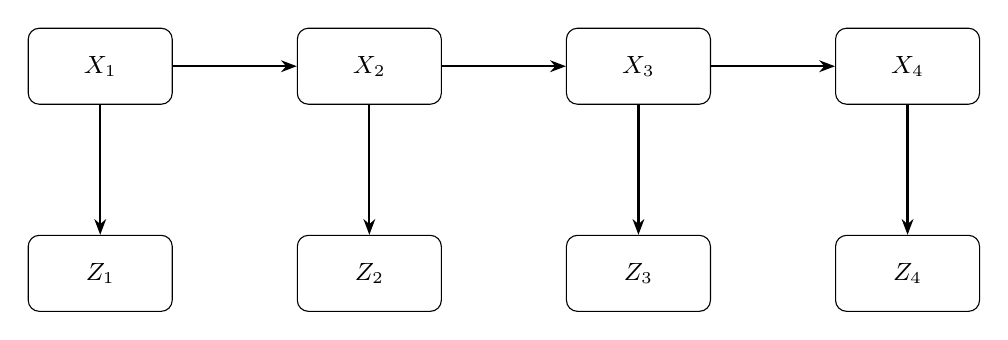
\begin{tikzpicture}[node distance=0.62in,every node/.style={draw,rounded corners,minimum width=0.72in,minimum height=0.38in,align=center,font=\small}]
      \node (x1) {$X_1$}; \node[right=of x1] (x2) {$X_2$}; \node[right=of x2] (x3) {$X_3$}; \node[right=of x3] (x4) {$X_4$};
      \node[below=0.65in of x1] (z1) {$Z_1$}; \node[below=0.65in of x2] (z2) {$Z_2$}; \node[below=0.65in of x3] (z3) {$Z_3$}; \node[below=0.65in of x4] (z4) {$Z_4$};
      \draw[-{Stealth[length=2mm]},thick] (x1)--(x2); \draw[-{Stealth[length=2mm]},thick] (x2)--(x3); \draw[-{Stealth[length=2mm]},thick] (x3)--(x4);
      \draw[-{Stealth[length=2mm]},thick] (x1)--(z1); \draw[-{Stealth[length=2mm]},thick] (x2)--(z2); \draw[-{Stealth[length=2mm]},thick] (x3)--(z3); \draw[-{Stealth[length=2mm]},thick] (x4)--(z4);
    \end{tikzpicture}
  \end{center}

  \begin{keyidea}
    HMMs are not a different universe from Bayesian networks; they are a restricted temporal Bayesian-network structure.
  \end{keyidea}
\end{frame}

% -----------------------------------------------------------------------------
% Slide 22
% -----------------------------------------------------------------------------
\begin{frame}[shrink=10]{The HMM Filtering Recursion}
  Prediction:
  \[
    P(X_t\mid z_{1:t-1})
    =\sum_{x_{t-1}}P(X_t\mid x_{t-1})P(x_{t-1}\mid z_{1:t-1}).
  \]

  Correction:
  \[
    P(X_t\mid z_{1:t})
    =\eta P(z_t\mid X_t)P(X_t\mid z_{1:t-1}).
  \]

  This is exactly the two-step filter we just used.

  \begin{keyidea}
    The HMM forward update compresses an arbitrarily long observation history into the current belief vector.
  \end{keyidea}
\end{frame}

% -----------------------------------------------------------------------------
% Slide 23
% -----------------------------------------------------------------------------
\begin{frame}[shrink=10]{Why This Avoids the History Explosion}
  Suppose the HMM has $n$ discrete states.

  We do \emph{not} retain all $n^{T+1}$ trajectories.

  We retain only
  \[
    bel_t=[P(X_t=s_1\mid z_{1:t}),\ldots,P(X_t=s_n\mid z_{1:t})].
  \]

  A dense transition update costs roughly
  \[
    O(n^2)
  \]
  per time step rather than enumerating all histories.

  \begin{keyidea}
    Dynamic programming works because many different histories lead to the same current state and can be merged into one probability mass.
  \end{keyidea}
\end{frame}

% -----------------------------------------------------------------------------
% Slide 24
% -----------------------------------------------------------------------------
\begin{frame}[shrink=10]{HMM Tradeoff: The State Must Be Good Enough}
  The Markov assumption is only useful if $X_t$ actually captures the information needed for future prediction.

  Bad state choice:
  \begin{itemize}
    \item omit velocity, and position may no longer predict next position well;
    \item omit sensor health, and observation errors may look inexplicable;
    \item omit crowd flow, and motion uncertainty may become strongly history-dependent.
  \end{itemize}

  \begin{keyidea}
    The price of Markov tractability is a state representation rich enough to make the future approximately conditionally independent of the distant past.
  \end{keyidea}
\end{frame}

% -----------------------------------------------------------------------------
% Slide 25
% -----------------------------------------------------------------------------
\begin{frame}[shrink=10]{HMMs Are Excellent When the Hidden State Is Discrete}
  Examples:
  \begin{itemize}
    \item robot is in one of a finite set of rooms;
    \item machine is in one of several health modes;
    \item user is in one of several activity states;
    \item speech system is in one of a sequence of phonetic states.
  \end{itemize}

  But our delivery robot's pose is not naturally
  \[
    \{A,B,C\}.
  \]

  It is closer to
  \[
    (x,y,\theta)\in\mathbb{R}^2\times[-\pi,\pi).
  \]

  \begin{keyidea}
    The next question is how to maintain a belief over a continuous state without discretizing the world into millions of bins.
  \end{keyidea}
\end{frame}

\section{Kalman Filtering: Continuous Gaussian Beliefs}

% -----------------------------------------------------------------------------
% Slide 26
% -----------------------------------------------------------------------------
\begin{frame}[shrink=10]{Why Not Just Discretize the Continuous Pose?}
  Suppose campus localization uses:
  \begin{itemize}
    \item 1000 possible $x$ bins;
    \item 1000 possible $y$ bins;
    \item 360 heading bins.
  \end{itemize}

  Then the pose grid already contains
  \[
    1000\times1000\times360=360{,}000{,}000
  \]
  discrete states.

  Before adding velocity, sensor bias, or anything else.

  \begin{keyidea}
    Fine discretization can recover continuous detail, but the state count explodes combinatorially.
  \end{keyidea}
\end{frame}

% -----------------------------------------------------------------------------
% Slide 27
% -----------------------------------------------------------------------------
\begin{frame}[shrink=10]{What If the Belief Has a Simple Shape?}
  Instead of storing every possible continuous state, suppose the belief is Gaussian:
  \[
    X_t\sim\mathcal{N}(\mu_t,\Sigma_t).
  \]

  Then the full belief is summarized by:
  \begin{itemize}
    \item a mean vector $\mu_t$;
    \item a covariance matrix $\Sigma_t$.
  \end{itemize}

  \lectureimage[1.7in]{slide27.png}

  \begin{keyidea}
    A parametric filter gains efficiency by assuming the belief can be represented with a small number of parameters.
  \end{keyidea}
\end{frame}

% -----------------------------------------------------------------------------
% Slide 28
% -----------------------------------------------------------------------------
\begin{frame}[shrink=10]{The Linear-Gaussian State-Space Model}
  Kalman filtering assumes linear dynamics with Gaussian noise:
  \[
    X_t=A X_{t-1}+B U_t+\epsilon_t,
    \qquad \epsilon_t\sim\mathcal{N}(0,Q).
  \]

  Measurements are also linear with Gaussian noise:
  \[
    Z_t=H X_t+\delta_t,
    \qquad \delta_t\sim\mathcal{N}(0,R).
  \]

  \begin{keyidea}
    Linear transformations of Gaussian variables remain Gaussian, so prediction and correction stay inside the same compact family.
  \end{keyidea}
\end{frame}

% -----------------------------------------------------------------------------
% Slide 29
% -----------------------------------------------------------------------------
\begin{frame}[shrink=10]{Kalman Filtering Is Still Predict Then Correct}
  \textbf{Predict:}
  \[
    \mu_t^- = A\mu_{t-1}+BU_t
  \]
  \[
    \Sigma_t^- = A\Sigma_{t-1}A^T+Q
  \]

  \textbf{Correct:}
  \[
    K_t=\Sigma_t^-H^T(H\Sigma_t^-H^T+R)^{-1}
  \]
  \[
    \mu_t=\mu_t^-+K_t(Z_t-H\mu_t^-)
  \]

  \begin{keyidea}
    The Kalman gain decides how strongly to trust the new measurement relative to the predicted uncertainty.
  \end{keyidea}
\end{frame}

% -----------------------------------------------------------------------------
% Slide 30
% -----------------------------------------------------------------------------
\begin{frame}[shrink=10]{One-Dimensional Kalman Example}
  Suppose before the measurement:
  \[
    X_t\sim\mathcal{N}(12,5).
  \]

  The position sensor reports
  \[
    z_t=11,
    \qquad R=4.
  \]

  Kalman gain:
  \[
    K=\frac{5}{5+4}=0.556.
  \]

  Updated mean:
  \[
    \mu_t=12+0.556(11-12)\approx11.44.
  \]

  Updated variance:
  \[
    \Sigma_t=(1-K)5\approx2.22.
  \]

  \begin{keyidea}
    The estimate moves toward the measurement, while uncertainty decreases because prediction and sensing provide complementary information.
  \end{keyidea}
\end{frame}

% -----------------------------------------------------------------------------
% Slide 31
% -----------------------------------------------------------------------------
\begin{frame}[shrink=10]{Why Kalman Filters Are So Attractive}
  \begin{itemize}
    \item continuous state without massive discretization;
    \item compact belief representation;
    \item recursive online updates;
    \item mathematically exact for the linear-Gaussian model;
    \item efficient matrix operations;
    \item natural fusion of multiple noisy measurements.
  \end{itemize}

  \begin{keyidea}
    Strong assumptions buy an unusually efficient and elegant state estimator.
  \end{keyidea}
\end{frame}

% -----------------------------------------------------------------------------
% Slide 32
% -----------------------------------------------------------------------------
\begin{frame}[shrink=10]{But the Gaussian Assumption Can Be the Wrong Shape}
  Imagine two visually identical campus corridors.

  The robot may plausibly be in either one.

  The belief is now \textbf{multimodal}:
  \[
    p(x)\approx \text{peak near corridor 1} + \text{peak near corridor 2}.
  \]

  One Gaussian tends to summarize that as a mean location \emph{between} the two possibilities.

  \lectureimage[1.65in]{slide32.png}

  \begin{keyidea}
    A compact parameterization can be computationally excellent while representing the wrong uncertainty geometry.
  \end{keyidea}
\end{frame}

% -----------------------------------------------------------------------------
% Slide 33
% -----------------------------------------------------------------------------
\begin{frame}[shrink=10]{Kalman Failure Modes Motivate a Different Representation}
  Standard Kalman filtering assumes:
  \begin{itemize}
    \item linear transition model;
    \item linear observation model;
    \item Gaussian process noise;
    \item Gaussian sensor noise;
    \item effectively unimodal belief.
  \end{itemize}

  Real localization can be nonlinear, asymmetric, and multimodal.

  \begin{keyidea}
    If the posterior cannot be represented well by one Gaussian, we need a belief representation that can take almost any shape.
  \end{keyidea}
\end{frame}

\section{Particle Filters: Sampling the Belief Over Time}

% -----------------------------------------------------------------------------
% Slide 34
% -----------------------------------------------------------------------------
\begin{frame}[shrink=10]{Lecture 20 Comes Back: Represent the Belief with Samples}
  A particle filter approximates the current belief with weighted samples:
  \[
    bel_t(x)\approx\{(x_t^{[1]},w_t^{[1]}),\ldots,(x_t^{[M]},w_t^{[M]})\}.
  \]

  Each particle is one hypothesis about the current state.

  Many particles in one region means high probability mass there.

  \lectureimage[1.75in]{slide34.png}

  \begin{keyidea}
    Particle filtering replaces one analytic distribution with a population of explicit state hypotheses.
  \end{keyidea}
\end{frame}

% -----------------------------------------------------------------------------
% Slide 35
% -----------------------------------------------------------------------------
\begin{frame}[shrink=10]{Particle Filtering: Predict, Weight, Resample}
  At each time step:
  \begin{enumerate}
    \item \textbf{Predict:} sample each particle through the motion model.
    \item \textbf{Weight:} score how well each predicted particle explains the observation.
    \item \textbf{Normalize:} convert scores into a probability distribution.
    \item \textbf{Resample:} preferentially copy high-weight particles and discard low-weight ones.
  \end{enumerate}

  \[
    w_t^{[i]}\propto P(z_t\mid x_t^{[i]}).
  \]

  \begin{keyidea}
    Particle filtering is sequential importance sampling plus resampling, applied repeatedly as evidence arrives.
  \end{keyidea}
\end{frame}

% -----------------------------------------------------------------------------
% Slide 36
% -----------------------------------------------------------------------------
\begin{frame}[shrink=10]{Why Resampling Matters}
  Without resampling, many particles eventually carry almost no weight.

  After resampling:
  \begin{itemize}
    \item hypotheses consistent with the sensor are duplicated;
    \item inconsistent hypotheses disappear;
    \item computation is concentrated where posterior probability is high.
  \end{itemize}

  \lectureimage[1.8in]{slide36.png}

  \begin{keyidea}
    Resampling reallocates a fixed computational budget toward the parts of state space that currently matter.
  \end{keyidea}
\end{frame}

% -----------------------------------------------------------------------------
% Slide 37
% -----------------------------------------------------------------------------
\begin{frame}[shrink=10]{Particle Filters Can Represent Multiple Hypotheses}
  Suppose the robot could be in either of two similar corridors.

  A particle set can maintain two clusters simultaneously.

  New sensor evidence may later eliminate one cluster.

  \begin{columns}[T,onlytextwidth]
    \begin{column}{0.47\textwidth}
      \begin{block}{Kalman belief}
        One Gaussian center + covariance.
      \end{block}
    \end{column}
    \begin{column}{0.47\textwidth}
      \begin{block}{Particle belief}
        Arbitrary shape, including multiple separated modes.
      \end{block}
    \end{column}
  \end{columns}

  \begin{keyidea}
    Particle filters trade analytic compactness for representational flexibility.
  \end{keyidea}
\end{frame}

% -----------------------------------------------------------------------------
% Slide 38
% -----------------------------------------------------------------------------
\begin{frame}[shrink=10]{Particle Filters Have Their Own Failure Modes}
  \begin{itemize}
    \item too few particles can miss important regions entirely;
    \item high-dimensional states may require very many particles;
    \item repeated resampling can reduce diversity;
    \item poor motion or sensor models still produce poor estimates;
    \item computation is stochastic rather than deterministic.
  \end{itemize}

  \begin{keyidea}
    Sampling avoids some analytic assumptions, but it pays with Monte Carlo variance and potentially large particle counts.
  \end{keyidea}
\end{frame}

\section{AMCL: The Robotics Payoff}

% -----------------------------------------------------------------------------
% Slide 39
% -----------------------------------------------------------------------------
\begin{frame}[shrink=10]{AMCL: Adaptive Monte Carlo Localization}
  In ROS 2 Navigation, AMCL is a particle-filter-based localizer for estimating robot pose in a known static map.

  It combines:
  \begin{itemize}
    \item a prior / current cloud of pose particles;
    \item odometry-based motion updates;
    \item laser-scan likelihoods against the map;
    \item resampling to concentrate hypotheses;
    \item an estimated pose distribution for navigation.
  \end{itemize}

  \begin{keyidea}
    AMCL is not just an abstract probability example: it operationalizes particle filtering for practical mobile-robot localization.
  \end{keyidea}
\end{frame}

% -----------------------------------------------------------------------------
% Slide 40
% -----------------------------------------------------------------------------
\begin{frame}[shrink=10]{What AMCL Is Estimating}
  The hidden state is approximately robot pose:
  \[
    X_t=(x_t,y_t,\theta_t).
  \]

  \begin{center}
    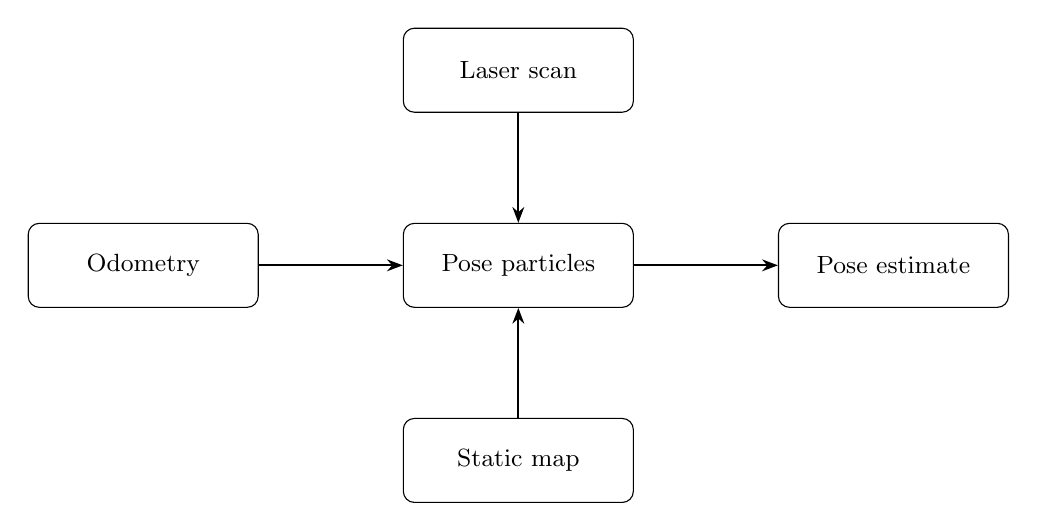
\begin{tikzpicture}[node distance=0.72in,every node/.style={draw,rounded corners,minimum width=1.15in,minimum height=0.42in,align=center,font=\small}]
      \node (odom) {Odometry};
      \node[right=of odom] (particles) {Pose particles};
      \node[above=0.55in of particles] (scan) {Laser scan};
      \node[below=0.55in of particles] (map) {Static map};
      \node[right=of particles] (pose) {Pose estimate};
      \draw[-{Stealth[length=2mm]},thick] (odom)--(particles);
      \draw[-{Stealth[length=2mm]},thick] (scan)--(particles);
      \draw[-{Stealth[length=2mm]},thick] (map)--(particles);
      \draw[-{Stealth[length=2mm]},thick] (particles)--(pose);
    \end{tikzpicture}
  \end{center}

  Evidence comes from a range sensor scored against a known map; motion information comes from odometry.

  \begin{keyidea}
    Localization is filtering: estimate current pose from motion history and sensor evidence without storing every past trajectory.
  \end{keyidea}
\end{frame}

% -----------------------------------------------------------------------------
% Slide 41
% -----------------------------------------------------------------------------
\begin{frame}[shrink=10]{One Problem, Three Belief Representations}
  \begin{columns}[T,onlytextwidth]
    \begin{column}{0.31\textwidth}
      \begin{block}{HMM}
        \small
        \textbf{State:} discrete\\
        \textbf{Belief:} probability vector\\
        \textbf{Exact?} yes, under the model\\
        \textbf{Multimodal?} yes, discrete\\
        \textbf{Cost:} state count\\
        \textbf{Assumption:} Markov + finite state
      \end{block}
    \end{column}
    \begin{column}{0.31\textwidth}
      \begin{block}{Kalman}
        \small
        \textbf{State:} continuous\\
        \textbf{Belief:} Gaussian $(\mu,\Sigma)$\\
        \textbf{Exact?} linear-Gaussian\\
        \textbf{Multimodal?} poorly\\
        \textbf{Cost:} matrix algebra\\
        \textbf{Assumption:} linear + Gaussian
      \end{block}
    \end{column}
    \begin{column}{0.31\textwidth}
      \begin{block}{Particle filter}
        \small
        \textbf{State:} general / continuous\\
        \textbf{Belief:} weighted samples\\
        \textbf{Exact?} approximate\\
        \textbf{Multimodal?} yes\\
        \textbf{Cost:} particle count\\
        \textbf{Assumption:} representative samples
      \end{block}
    \end{column}
  \end{columns}

  \begin{keyidea}
    The filtering idea is shared; the algorithms differ mainly in how they represent and update the belief distribution.
  \end{keyidea}
\end{frame}

% -----------------------------------------------------------------------------
% Slide 42
% -----------------------------------------------------------------------------
\begin{frame}[shrink=10]{The Whole Lecture in One Flow}
  \begin{enumerate}
    \item Static Bayesian network: reason about one snapshot.
    \item Dynamic Bayesian network: repeat structure through time.
    \item Filtering: maintain $P(X_t\mid z_{1:t})$ online.
    \item Markov assumption: summarize relevant history in the current state belief.
    \item Choose a belief representation appropriate to the problem.
  \end{enumerate}

  \begin{columns}[T,onlytextwidth]
    \begin{column}{0.30\textwidth}
      \begin{block}{HMM}
        \centering Discrete state\\Probability vector
      \end{block}
    \end{column}
    \begin{column}{0.30\textwidth}
      \begin{block}{Kalman}
        \centering Continuous state\\Gaussian belief
      \end{block}
    \end{column}
    \begin{column}{0.30\textwidth}
      \begin{block}{Particle filter}
        \centering General state\\Weighted samples
      \end{block}
    \end{column}
  \end{columns}

  \begin{keyidea}
    State estimation is a sequence of tradeoffs: what state to remember, what uncertainty shape to assume, and how much computation to spend.
  \end{keyidea}
\end{frame}

% -----------------------------------------------------------------------------
% Slide 43
% -----------------------------------------------------------------------------
\begin{frame}[shrink=10]{Takeaways}
  \begin{itemize}
    \item Dynamic Bayesian networks extend probabilistic graphical models across time.
    \item Filtering recursively combines a transition model with new evidence.
    \item Explicit state histories explode; the Markov assumption lets the current belief summarize the relevant past.
    \item HMMs provide exact filtering for compact discrete hidden states.
    \item Kalman filters compress continuous linear-Gaussian beliefs into a mean and covariance.
    \item Particle filters approximate flexible, multimodal beliefs with weighted samples.
    \item AMCL applies particle filtering to practical map-based mobile-robot localization.
  \end{itemize}

  \begin{keyidea}
    The central engineering question is not ``which filter is best?'' It is ``which representation of uncertainty matches the structure of this state-estimation problem?''
  \end{keyidea}
\end{frame}

\end{document}
